\documentclass[%
 reprint,
%superscriptaddress,
%groupedaddress,
%unsortedaddress,
%runinaddress,
%frontmatterverbose, 
%preprint,
%showpacs,preprintnumbers,
%nofootinbib,
%nobibnotes,
%bibnotes,
 amsmath,amssymb,
 aps,
 pra,
%prb,
%rmp,
%prstab,
%prstper,
%floatfix,
]{revtex4-1}

\usepackage{graphicx}% Include figure files
\usepackage{dcolumn}% Align table columns on decimal point
%\usepackage{bm}% bold math
\usepackage{fullpage}
\usepackage{epsfig}
\usepackage{amsmath}
\usepackage{amsfonts}
\usepackage{amssymb}
\usepackage{float}
\usepackage{pstricks}
\usepackage{cancel}
\usepackage{lipsum}
%\usepackage[nottoc,numbib]{tocbibind} %Uncomment for bibliography to be its own numbered section
\usepackage{units}
\usepackage{listings}

\begin{document}

\preprint{APS/123-QED}

\title{\textbf{Lab Report: Compton Scattering} \\ \small{And Investigation of the Angular Dependence of the Scattering Probability for Photons}}
\author{Joshua LaBounty}
\author{Thomas Krahulik}
\affiliation{%
Stony Brook University --- PHY 445
}%

\date{\today}

\begin{abstract}
	In this experiment, we perform an investigation of the Compton Effect
\end{abstract}
\maketitle

\section{Background}

\begin{gather}\label{eq:energy_scatter}
	E_\gamma ' = \frac{E_\gamma}{1 + \frac{E_\gamma}{m_e c^2} (1 - \cos{\theta})}
\end{gather}

\begin{equation}\label{eq:thompson}
	\frac{d \sigma}{d \Omega}_{Th} = \frac{r_0^2}{2}(1+\cos^2{\theta})
\end{equation}

\begin{gather}\label{eq:kn}
	\frac{d \sigma}{d \Omega}_{KN} = \frac{r_0^2}{2} \frac{1 + \cos^2{\theta}}{[1 + \gamma(1 - \cos{\theta})]^2} \nonumber * ~~~~~~~~~~~~\\
	\left[ 1 + \frac{\gamma^2(1 - \cos{\theta})^2}{(1 + \cos^2{\theta})(1+ \gamma(1 - \cos{\theta}))}\right] 
\end{gather}

\section{Review of Previous Work}

\section{Experimental Setup}

\section{Measurements}

\subsection{Calibration of Detector Energy Scale}

\subsection{Electron Mass}

\subsection{Angular Dependence of the Scattering Probability}

\subsection{Free Electrons in Cu and Al}

\section{Theoretical Model}

\section{Comparison of Theory and Experiment}

\section{Discussion and Conclusions}

\section{Author Contributions}

\begin{thebibliography}{4}
	
	\bibitem{milissinos}
	A.C. Melissinos, Experiments in Modern Physics (Academic Press, NY, 1966).
	
	\bibitem{bevington}
	Philip R. Bevington and D. Keith Robinson, Data Reduction and Error Analysis 3rd edition (McGraw-Hill, 2003).
	
	\bibitem{compton_paper_original}
	A. H. Compton, Phys. Rev. 21 , 483 and 715 (1923).
	
	\bibitem{bartlett}
	A. A. Bartlett, Am. J. Phys. 32 , 120 (1964).

\end{thebibliography}

\begin{appendix}

\section{Derivation of Equation \ref{eq:energy_scatter}}

\begin{figure}[H]
	\centering
	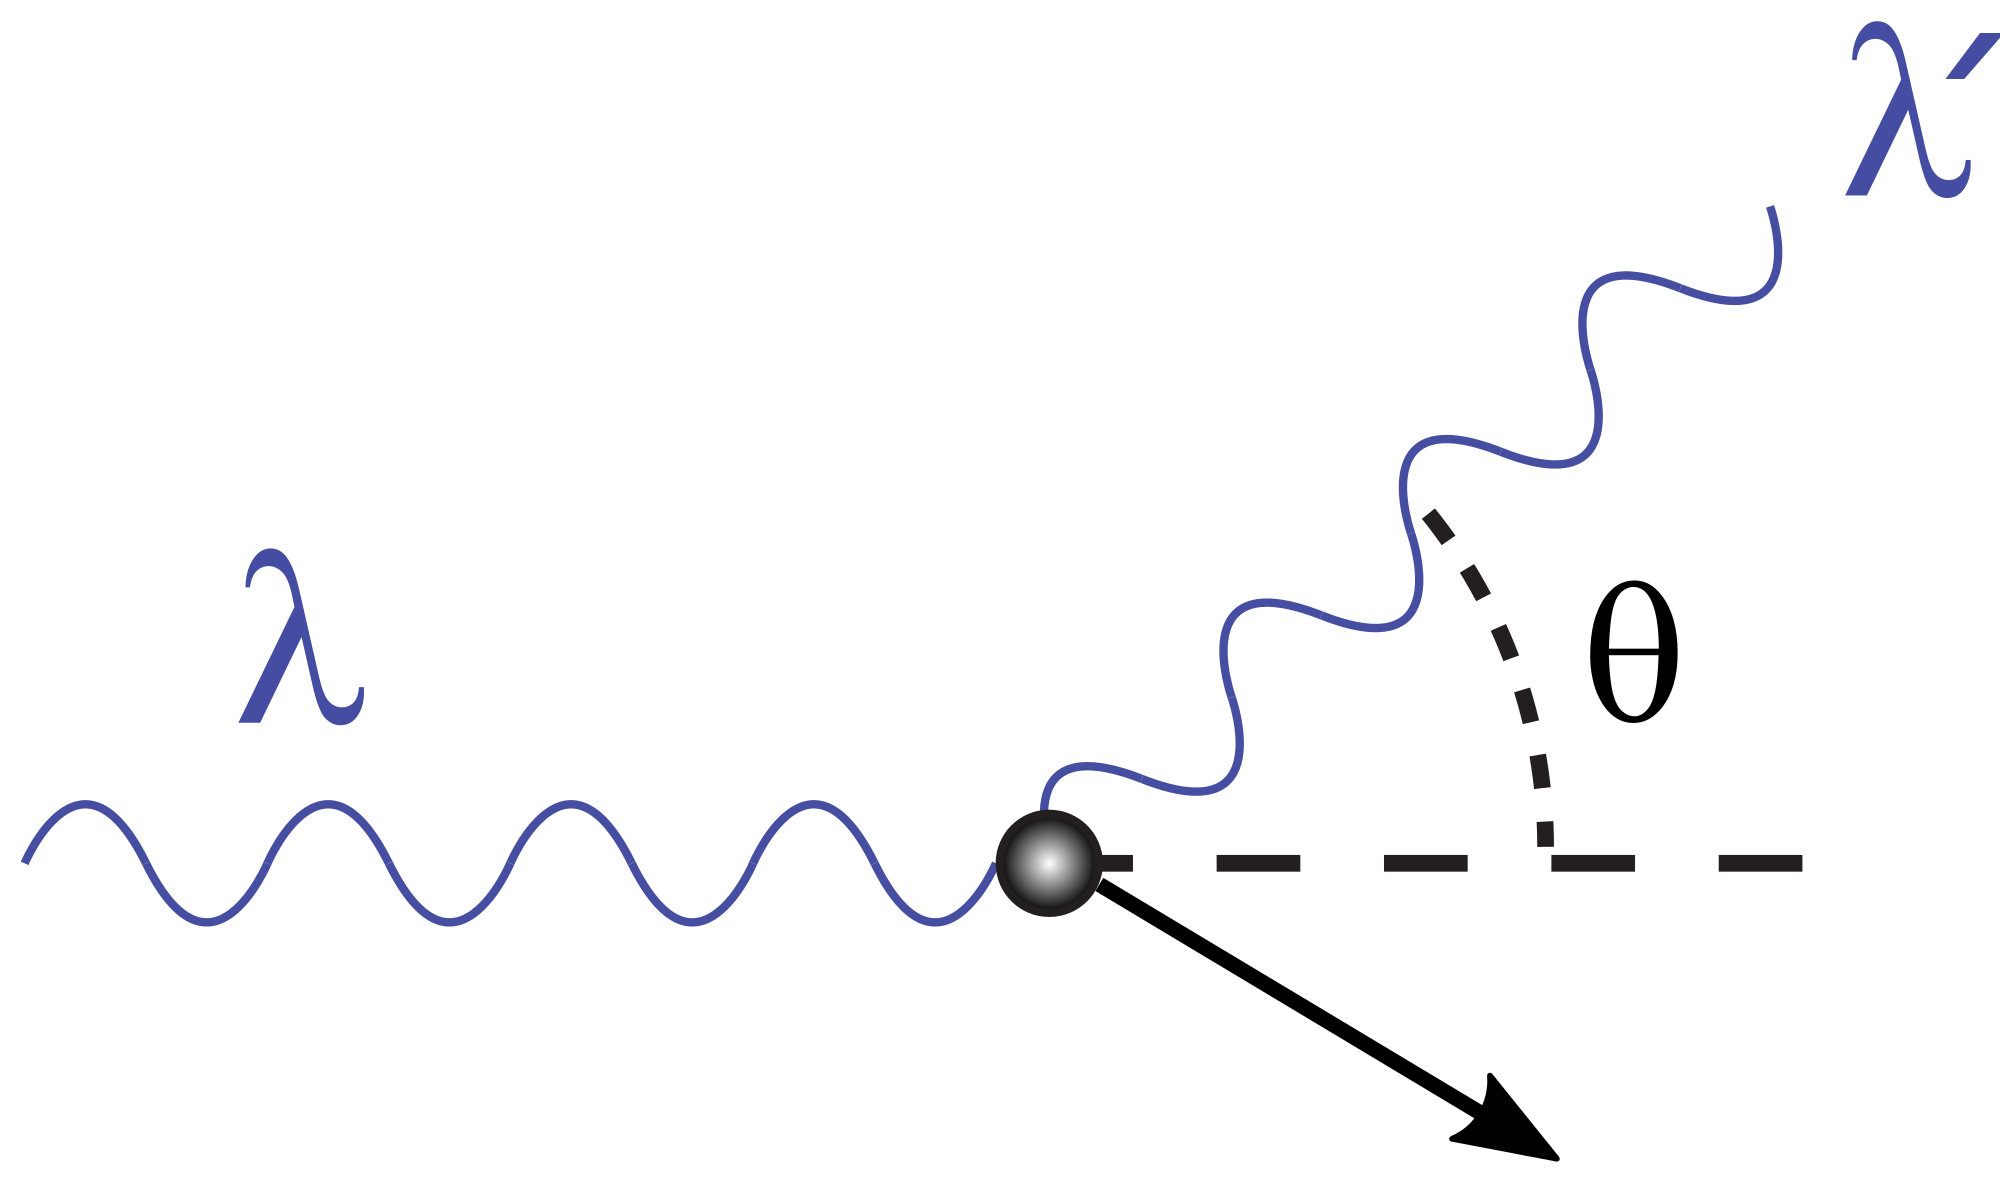
\includegraphics[width=0.3\textwidth]{../plots/ComptonDiagram.png}
	\caption{Diagram showing a photon scattering off an electron at rest. Image courtesy of Wikipedia.}
\end{figure}

This formula can be described semi-classically using only conservation of energy and conservation of momentum. We approximate this interaction as a photon impacting an electron which is currently at rest. The conservation laws require that:

\begin{gather}
	E_\gamma + E_e = E_\gamma ' + E_e '\nonumber \\
	\mathbf{p}_\gamma = \mathbf{p}_\gamma' + \mathbf{p}_e' \nonumber
\end{gather}
Initially:
\begin{gather}
	E_e = m_e c^2 \nonumber
\end{gather}
And after the collision:
\begin{gather}
	E_e' = \sqrt{(\mathbf{p}_e' c)^2 + (m_e c^2)^2} \nonumber
\end{gather}
Substituting these quantities into conservation of energy, we find:
\begin{gather}
	E_\gamma + m_e c^2 = E_\gamma' + \sqrt{(\mathbf{p}_e' c)^2 + (m_e c^2)^2} \nonumber \\
	\downarrow \nonumber \\
	\mathbf{p}_e^{2'} c^2  = (E_\gamma - E_\gamma' + m_e c^2)^2 - m_e^2 c^4 \nonumber
\end{gather}
Now returning to conservation of momentum:
\begin{gather}
	\mathbf{p}_e' = \mathbf{p}_\gamma - \mathbf{p}_\gamma' \nonumber
\end{gather}
Since these momenta are vector quantities, and we are only interested in a scalar, we can take the dot product:
\begin{gather}
	p_e^{2'} = \mathbf{p}_e' \cdot \mathbf{p}_e' = p_\gamma^2 + p_\gamma^{2'} - 2 p_\gamma p_\gamma' \cos{\theta} \nonumber \\
	p_e^{2'} c^2 =  p_\gamma^2 c^2 + p_\gamma^{2'} c^2 - 2 c^2 p_\gamma p_\gamma' \cos{\theta} \nonumber \\
	p_e^{2'} c^2 = E_\gamma^2 + E_\gamma^{2'} - 2 E_\gamma E_\gamma' \cos{\theta} \nonumber
\end{gather}
We can now equate these two equations for $p_e^{2'} c^2$ and find:
\begin{gather}
	(E_\gamma - E_\gamma' + m_e c^2)^2 - m_e^2 c^4 = E_\gamma^2 + E_\gamma^{2'} - 2 E_\gamma E_\gamma' \cos{\theta} \nonumber
\end{gather}
We then complete the square and reduce this equation in order to find:
\begin{gather}
	2 m_e c^2 (E_\gamma - E_\gamma') = 2 E_\gamma E_\gamma' (1- \cos{\theta}) \nonumber
\end{gather}
Which we rearrange to arrive back at Equation \ref{eq:energy_scatter}:
\begin{gather}
	E_\gamma ' = \frac{E_\gamma}{1 + \frac{E_\gamma}{m_e c^2} (1 - \cos{\theta})} \nonumber
\end{gather}

\end{appendix}

\end{document}


































